
\documentclass[11pt,oneside]{article} 

\usepackage{a4wide}

\usepackage{amsmath}
\usepackage{color}
%\usepackage{natbib} % kills arxiv 
\usepackage{framed}
%\usepackage{cite}
\usepackage{tikz}
\usepackage{tikz-cd}

\RequirePackage{amsmath}
\RequirePackage{amssymb}
\RequirePackage{amsthm}
%\RequirePackage{algorithmic}
%\RequirePackage{algorithm}
%\RequirePackage{theorem}
%\RequirePackage{eucal}
\RequirePackage{color}
\RequirePackage{url}
\RequirePackage{mdwlist}

\RequirePackage[all]{xy}
%\_CompileMatrices
%\RequirePackage{hyperref}
\RequirePackage{graphicx}
%\RequirePackage[dvips]{geometry}

\usepackage{xcolor}
\usepackage{amsmath,amsfonts,amssymb}
\usepackage{graphicx}
\usepackage[caption=false]{subfig}
\usepackage{enumerate}
\usepackage{mathrsfs}

% -------------- Commands ----------------------

\newcommand{\Eref}[1]{(\ref{#1})}
\newcommand{\Fref}[1]{Fig.~\ref{#1}}
%\newcommand{\Aref}[1]{Appendix~\ref{#1}}
\newcommand{\SRef}[1]{Section~\ref{#1}}

\newcommand{\todo}[1]{\ \textcolor{red}{\{#1\}}\ }

\newcommand{\Aut}{\mathrm{Aut}}
\newcommand{\Hom}{\mathrm{Hom}}
\newcommand{\Stab}{\mathrm{Stab}}
\newcommand{\Fix}{\mathrm{Fix}}
\newcommand{\Orbit}{\mathrm{Orbit}}
\newcommand{\Ker}{\mathrm{Ker}}
\newcommand{\Image}{\mathrm{Im}}
\newcommand{\Dim}{\mathrm{Dim}}
\newcommand{\Complex}{\mathbb{C}}
\newcommand{\GL}{\mathrm{GL}}
\newcommand{\Field}{\mathbb{F}}

% Lemma, proof, theorem, etc.
\newcommand\nounderline[1]{ #1} 
\newcommand\dolemma[1]{\vskip 5pt \noindent{\bf \underline{Lemma #1.}\ }}
\newcommand\doproposition[1]{\vskip 5pt \noindent {\bf \underline{Proposition #1.}\ }}
\newcommand\dotheorem[1]{\vskip 5pt \noindent {\bf \underline{Theorem #1.}\ }}
\newcommand\docorollary[1]{\vskip 5pt \noindent {\bf \underline{Corollary #1.}\ }}
\newcommand\doexample[1]{\vskip 5pt \noindent {\bf \underline{Example #1.}\ }}
\newcommand\doproof{\vskip 5pt \noindent{\bf \nounderline{Proof:}\ }}

\newcommand\tombstone{\rule{.36em}{2ex}\vskip 5pt}

\newcounter{numitem}
\newcommand{\numitem}[1]{\refstepcounter{numitem}\thenumitem\label{#1}}

% braket notation...
\newcommand{\ket}[1]{|{#1}\rangle}
\newcommand{\expect}[1]{\langle{#1}\rangle}
\newcommand{\bra}[1]{\langle{#1}|}
\newcommand{\ketbra}[2]{\ket{#1}\!\bra{#2}}
\newcommand{\braket}[2]{\langle{#1}|{#2}\rangle}

% Categories
\newcommand{\Set}{\mathbf{Set}}
\newcommand{\FinSet}{\mathbf{FinSet}}
\newcommand{\GSet}{\mathbf{GSet}}
\newcommand{\GRep}{\mathbf{GRep}}

\newcommand{\thinplus}{\!+\!}

\renewcommand{\arraystretch}{1.2}



\title{Notes on Hecke Operators}

\author{Simon Burton}


\date{\today}

\flushbottom

\begin{document}

\maketitle

%\begin{abstract}
%\end{abstract}

%\tableofcontents

%\doublespacing
%\onehalfspacing

\section{Introduction}

Group representation theory concerns itself with
homomorphisms from a group $G$ to the general
linear group over a field $k:$
$$
    G \to \GL(n, k).
$$
The definition of the general linear group
makes sense not just for
a field $k$, but also for a ring, or even a 
semi-ring (a ring without additive inverses.)
In particular, we consider 
the semi-ring of truth-values:
$$
    \Field_1 = \{\mathrm{false}, \mathrm{true}\}
$$
with addition as disjunction and multiplication
as conjunction.
The notation $\Field_1$ refers to the ``field
with one element'',
which however is not a field and doesn't have one element \cite{Lorscheid2018}. 
We have the following
\dotheorem{\numitem{F1thm}}
The group $\GL(n, \Field_1)$ consists of $n\times n$
permutation matrices, and is therefore isomorphic
to the permutation group $S_n$.
\doproof
Adapted from \cite{Speyer2011}.
\tombstone

And so we find that group representation theory over the
semi-ring of truth values is the theory of groups acting on sets.

\section{Groups acting on sets}

We say a group $G$ \emph{acts} on a set $X$ when there
is a group homomorphism:
$$
    G \to \Aut(X).
$$
We choose not to name this homomorphism, and instead
confuse the elements of $G$ with their image in $\Aut(X).$
In this way we understood expressions such as $gx$ for $g\in G, x\in X.$
This is similar to how a field acts on a vector space:
we don't usually write the homomorphism, and instead just
let elements of the field act on the vectors (on the left.)

We also call this setup a $G$-set $X$.

%A map from a group action $G\to\Aut(X)$ to $G\to\Aut(Y)$
A map of $G$-sets $X\to Y$
is a set function $f:X\to Y$ that commutes with the group action.
That is, for every $g\in G$ we have the commuting square:
\[
\begin{tikzcd}
 X \arrow{d}{f} \arrow{r}{g} &  X \arrow{d}{f} \\
 Y \arrow{r}{g} &  Y 
\end{tikzcd}
\]
Thinking of $G$ as a one object category, a group action is
then a set-valued functor and we see that a map of $G$-sets
is the same as a natural transformation of functors.
This gives the category of $G$-sets which we denote $\GSet.$

For $x\in X$ the \emph{stabilizer} is defined
$$
    \Stab(x) := \{ g\in G \ | \ gx = x \}.
$$
This is clearly a subgroup of $G$.
Dually, 
the \emph{fixed point set} of $g\in G$
is the subset of $X$ given by
$$
    \Fix(g) := \{ x\in X \ | \ gx = x \}.
$$
\todo{In what sense are these really dual?}

The \emph{orbit} of $x\in X$ is the set
$$
    \Orbit(x) := \{ gx \ | \ g\in G \}.
$$

A simple calculation shows that the stabilizers of
points in the same orbit are related by conjugation:
given a $G$-set $X$, with $x\in X, g\in G$, we have
$$
    \Stab(gx) = g\Stab(x) g^{-1}.
$$

Given an arbitrary group $G$, 
there are many ways to cook up a set that $G$ acts on.
The most important such recipe is the following.
Let $H$ be any subgroup of $G$,
and let $X=\{gH\}_{g\in G}$ be the set of left cosets of $H$.
Then $G$ acts on $X$ by left-multiplication,
and this action is transitive.
We get the \emph{left regular action} when $H=\{1\}$ and
we get the trivial action when $H=G.$
But this recipe has a converse:
any transitive $G$-set $X$ is
isomorphic to a $G$-set $\{gH\}_{g\in G}$ for
some subgroup $H\in G.$
The subgroup can be chosen to be the
stabilizer of any point $x\in X.$

We now state the \emph{orbit-stabilizer theorem}.
\dotheorem{\numitem{thmOS}}%{\bf (orbit-stabilizer)}
Given a $G$-set $X$ and a point $x\in X$
there is a bijection of sets:
$$
    \Orbit(x) \times \Stab(x) \cong G.
$$

\doproof
Let $H$ be the subgroup
$$
    H = \Stab(x).
$$
Then $G$ is partitioned into cosets $\{gH\ |\ g\in G\}.$
We claim that this set of cosets is in bijection with
the orbit of $x$,
with bijection given by the relation
\begin{align*}
    \Orbit(x) &\to \{gH \ |\ g\in G\} \\
    gx  &\mapsto  gH.
\end{align*}
To show that this relation is actually a function,
let $gx=hx$ for $g,h\in G.$
Then $h^{-1}gx = x$ and so $h^{-1}g\in H,$
and the cosets $gH$ and $hH$ are identical.
\todo{finish}
\tombstone

% https://math.stackexchange.com/questions/1659075/category-theoretic-relation-between-orbit-stabilizer-and-rank-nullity-theorems/2168381
\doexample{\numitem{exvec}}
The rank-nullity theorem says that given
a linear map on finite-dimensional vector spaces $A:V\to V$,
$$
    \Dim(\Image(A)) + \Dim(\Ker(A)) = \Dim(V).
$$
Such a map gives a group action:
it is the additive group of $V$ acting on the set $V$
by addition. That is, any $v\in V$ acts on $x\in V$ as
$v: x \mapsto x+Av.$ 
Now we see that given any $x\in V$ the stabilizer subgroup
$\Stab(x)$ of this action is precisely the kernel
of $A.$ The orbit of $x$ is $x$ plus the image of $A.$

Working with a vector space over a finite field,
we can take the cardinality of these sets as in the formula
$|\Orbit(x)||\Stab(x)| = |G|$ and 
take the logarithm of this where the base is
the size of the field and we get exactly the rank-nullity
equation.

Over an infinite field this doesn't work and
we need to think more along the lines of a categorified
orbit-stabilizer theorem. 
\todo{Does this really work?}
In this case, for each $x\in
V$ we can find a bijection:

$$
\Orbit(x) \cong G / \Stab(x)
$$
and this bijection gives us the First Isomorphism Theorem:
$$
\Image(A) \cong V / \Ker(A). 
$$ 
\todo{Question: 
Can we bootstrap this one more time in order
to say something about the size of the homology 
groups in a chain complex?
Perhaps thinking of a (length 2) 
chain complex as a 2-category?}
\tombstone

For a $G$-set $X$, the \emph{orbit space} is defined as
the set of orbits:
$$
    G\backslash X := \{\Orbit(x)\}_{x\in X}.
$$

The following is known as ``Burnside's lemma''.
\dotheorem{\numitem{thmBurnside}}%{\bf (Burnside's lemma)}
Given a $G$-set $X$,
$$
    |G\backslash X| = \frac{1}{|G|} \sum_{g\in G} | \Fix(g) |.
$$
\doproof
\todo{todo}
\tombstone

An action is \emph{faithful} when for each $g\in G$ with
$g\ne 1$ we have $\Fix(g)\ne X.$
An action is \emph{free} when for each $g\in G$ with
$g\ne 1$ we have $\Fix(g)=\phi.$

\todo{define a torsor}

A $G$-set with only one orbit is called \emph{simple} 
(or \emph{transitive}, or \emph{indecomposable}).

Given two $G$-sets $X$ and $Y$, we define the sum $X+Y$ 
\todo{...} and the product $X\times Y$ \todo{...}

The following theorem shows that 
$G$-sets are semi-simple.
\dotheorem{\numitem{F1semisimple}}
For a $G$-set $X$, we have
$$
    X = \sum_{i=1}^{n} X_i
$$
with $X_i$ simple, and the summation is unique up to reordering.
\doproof
Easy.
\tombstone

The next theorem is a kind of ``Schur's lemma for $G$-sets''.
\dotheorem{\numitem{F1schur}}
Given $G$-sets $X$ and $Y$:

(a) For $f:X\to Y,$ we have $f(X)$ is a $G$-set, $f(X)\subseteq Y.$

(b) For $f:X\to Y,$ and $X\ne\phi$,
if $Y$ is simple then $f$ is surjective.

(c) For $f:X\to X$ with $X$ simple, $f$ is an automorpism.

\doproof
Easy.
\tombstone

\subsection{The category of canonical orbits}

Taken from \cite{Bredon2006,Dress1971}.

\subsection{Double cosets}

Given a map of sets $f:X\to Y$, 
that is \emph{$G$-invariant}
ie., $f(x)=f(gx)$ for all $g\in G, x\in X$,
we can \emph{lift} to a unique map $\tilde{f}: G\backslash X\to Y$ such that
\[
\begin{tikzcd}
 X \arrow{rd}{p} \arrow{r}{f} &  Y \\
  &  G\backslash X \arrow{u}{\tilde{f}} 
\end{tikzcd}
\]
where $p$ is the projection map $p:X\to G\backslash X.$
We use this observation in the proof of the following.

\doproposition{\numitem{propdcoset}}
Given a group $G$ with subgroups $H$ and $K$,
the orbit-space of the $G$-set $G/H~\times~G/K$ is in bijection
with the $H,K$ double cosets:
$$
    G\backslash(G/H\times G/K) \cong \{ HgK \}_{g\in G}.
$$
\doproof
We will show that the following relation
\begin{align*}
f : G/H\times G/K &\to \{HgK\}_{g\in G} \\
    f(aH, bK) &:= Ha^{-1}bK,
\end{align*}
defines a $G$-invariant function that lifts
to the required bijection on the orbits.

(i) That $f$ defines a function:
for any $h\in H, k\in K$,
$f(aH,bK)=Ha^{-1}bK=H(h^{-1}a^{-1})(bk)K=f(ahH,bkK).$

(ii) That $f$ is $G$-invariant: 
$f(gaH, gbK) = Ha^{-1}g^{-1}gbK = f(aH, bK)$.

(iii) $f$ is surjective, and so the lift $\tilde{f}$,
\[
\begin{tikzcd}
 G/H\times G/K \arrow{rd}{p} \arrow{r}{f} &  Y \\
  &  G\backslash (G/H\times G/K) \arrow{u}{\tilde{f}} 
\end{tikzcd}
\]
is also surjective.

(iv) That $\tilde{f}$ is injective,
\begin{align*}
    f(aH, bK) &= f(cH, dK) \ \ \mathrm{iff} \\
    Ha^{-1}bK &= Hc^{-1}dK \ \ \mathrm{iff}  \\
    \exists h,k\in G,\  a^{-1}b &= hc^{-1}dk \ \ \mathrm{iff} \\
    b &= (ahc^{-1})dk \ \ \mathrm{iff} \\
    bK = gdK,\ \  & aH = gcH, \ \ \mathrm{where}\ \  g=ahc^{-1} 
\end{align*}
And so $(aH, bK)$ and $(cH, dK)$ are in the same orbit.
\tombstone


\doproposition{\numitem{propfinestmut}}
\todo{Not sure how this goes exactly...}
Let $G$ be a group, with subgroups $H$ and $K$.
Considered as an equivelance relation on the
elements of $G$, the set of double cosets $\{HgK\}_{g\in G}$
is the finest mutual coarsening of the equivelance
relations given by the right and left cosets,
$\{Hg\}_{g\in G}$ and $\{gK\}_{g\in G}.$
In other words, as equivelance relations we have
$$
\{HgK\}_{g\in G} = \{Hg\}_{g\in G} \vee \{gK\}_{g\in G}.
$$
\doproof
\todo{todo}
\tombstone


\subsection{Hecke operators}

Let $\Complex[X]$ denote the complex vector space with basis $X.$
Evidently, when $X$ is a $G$-set, we get a $\Complex$-linear
representation of $G$ on $\Complex[X].$
A $\Complex$-linear representation of $G$ obtained in this
way we call a \emph{permutation representation}.

Given a point $x\in X$ we denote the corresponding basis
vector in $\Complex[X]$ as $\ket{x},$
and corresponding dual vector as $\bra{x}.$
We also denote generic vectors in $\Complex[X]$ by $\ket{v}$, $\ket{u}$, etc.

Given $G$-sets $X$ and $Y$, and points $x\in X, y\in Y$
we define the \emph{Hecke operator} as the linear operator
$$
    \Complex[X] \overset{r_{x,y}}{\longrightarrow} \Complex[Y]
$$
given by
$$
    r_{x,y} := \frac{1}{|\Stab(x)||\Stab(y)|} 
    \sum_{g\in G} \ket{gy}\bra{gx}.
$$

\dolemma{\numitem{lemmaHecke1}}
The Hecke operators are $G$-rep homomorphisms:
$$
    r_{x,y} \in \Hom_{\GRep}(\Complex[X], \Complex[Y]).
$$

\doproof
We need to show that 
$gr_{x,y}\ket{v} = r_{x,y} g\ket{v}$ for $\ket{v}\in\Complex[X], g\in G.$
By linearity we need only consider this equation on basis vectors:
$gr_{x,y}\ket{x'} = r_{x,y} g\ket{x'}$ for $x'\in X, g\in G.$
Computing:
\begin{align*}
    \mathrm{LHS} &= g\sum_{h\in H} \ket{hy} \\
     &= \sum_{h\in H} gh \ket{y} \\
    \mathrm{RHS} &= \sum_{h\in G} \ket{hy}\braket{hx}{gx} \\
     &= \sum_{h\in G, hx=gx} \ket{hy}\\
     &= \sum_{h\in H} gh \ket{y}.
\end{align*}
\todo{what is $H$?}
\tombstone


\dotheorem{\numitem{thm1}}
Given two permutation representation $\Complex[X]$
and $\Complex[Y]$ of a group $G$,
the Hecke operators
$$
    \{ r_{x,y} \ | \ x\in X, y\in Y \}
$$
form a basis for the linear space
$$
\Hom_{\GRep}(\Complex[X], \Complex[Y]).
$$

\doproof
Let $f\in \Hom_{\GRep}(\Complex[X], \Complex[Y]).$
Then for any $g\in G, x\in X, y\in Y$ we have:
\begin{align*}
    gf\ket{x} &= fg\ket{x} \\ 
    f\ket{x} &= g^{-1}fg\ket{x} \\ 
    \bra{y}f\ket{x} &= \bra{y}g^{-1}fg\ket{x} \\ 
              &= \bra{gy}f\ket{gx}.
\end{align*}
ie., the matrix for $f$ is constant on the orbits of
$X\times Y$ and so $f$ is a sum of Hecke operators.
\tombstone

\docorollary{\numitem{Hecke2}}
Given a doubly transitive action $G\to\Aut(X)$
the permutation representation $\Complex[X]$
breaks into exactly two irreducible representations. % in $\GRep.$
\doproof
There are two Hecke operators corresponding to the
diagonal matrix, and the off-diagonal matrix.
The result follows by the previous theorem and Schur's lemma.
\tombstone

\section{Kleinien geometry}

Given a homogeneous ``space'' $X$ 
the idea is to refer to, or define, geometric 
figures (a ``line'' or ``point'', etc.)
by the subgroup that fixes that figure.
%This is essentially the same idea as in Galois theory, 

\begin{center}
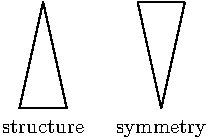
\includegraphics[]{pic-structure.pdf} 
\end{center}

\subsection{Example: the triangle}

This is about the simplest example that has
some substance to it.
Because it is our first example we go into
great detail.

We consider the group $G = S_3$ 
acting as the permutation group on three things.
Enumerating these three things, we write
the elements of $S_3$ according to their
action:
$$
    S_3 = \bigl\{ (1)(2)(3), (1)(23), (13)(2), (12)(3), (123), (132) \bigr\}.
$$

This group acts by isometries on the equi-angle triangle:
\begin{center}
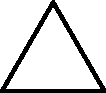
\includegraphics[]{pic-triangle.pdf} 
\end{center}
but we can only ``see'' this action if we add some
\emph{structure}. 
For example, we can number the
points (vertices) of the triangle:
\begin{center}
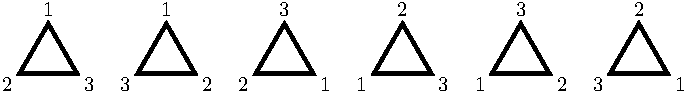
\includegraphics[]{pic-triangle-numbered.pdf} 
\end{center}
We call this kind of structure a \emph{frame}
because it allows us to see everything that is going on
with the group action.

Here we do the same, but instead of numbering the points
we shade a portion of the interior.
This is a more graphical depiction of a frame.
\begin{center}
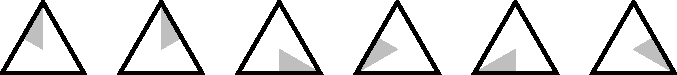
\includegraphics[]{pic-triangle-frames.pdf} 
\end{center}
By shading a different portion we find the structure
corresponding to a \emph{point}:
\begin{center}
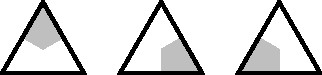
\includegraphics[]{pic-triangle-points.pdf} 
\end{center}
There is one other structure which we call an \emph{orientation}:
\begin{center}
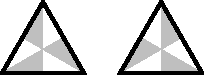
\includegraphics[]{pic-triangle-orientations.pdf} 
\end{center}

Using the Kleinien perspective, we associate
each of these structures with the subgroup of $G$
that stabilizes the structure.
And vice-versa: every subgroup of $G$ corresponds
to some kind of structure.

%\begin{samepage}
%%\underline{title }
%\begin{center}
%\begin{tabular}{ |c|l| }
%\hline
%structure & stabilizer subgroup, other cosets           \\
%\hline
%nothing   & $\bigl\{(1)(2)(3), (1)(23), (13)(2), (12)(3), (123), (132) \bigr\}$ \\
%\hline
%orientation   & $\bigl\{(1)(2)(3), (123), (132)\bigr\}, \ \bigl\{ (1)(23), (13)(2), (12)(3)\bigr\}$ \\
%\hline
%point  & $\bigl\{(1)(2)(3), (1)(23) \bigr\}, \ \bigl\{(13)(2), (123)\bigr\}, \ \bigl\{(12)(3), (132)\bigr\} $ \\
%\hline
%"  & $\bigl\{(1)(2)(3), (13)(2) \bigr\}, \ \bigl\{ (1)(23), (132) \bigr\}, \ \bigl\{(12)(3), (123)\bigr\} $ \\
%\hline
%"  & $\bigl\{(1)(2)(3), (12)(3) \bigr\}, \ \bigl\{ (13)(2), (132) \bigr\}, \ \bigl\{(1)(23), (123)\bigr\} $ \\
%\hline
%frame   & $\bigl\{(1)(2)(3)\bigr\}, \ \bigl\{ (1)(23)\bigr\}, \ \bigl\{ (13)(2)\bigr\}, \ \bigl\{ (12)(3)\bigr\}, \ \bigl\{ (123)\bigr\}, \ \bigl\{ (132) \bigr\}$ \\
%\hline
%\end{tabular}
%\end{center}
%\end{samepage}

%\begin{samepage}
%%\underline{title }
%\begin{center}
%\begin{tabular}{ |c|l| }
%\hline
%structure & stabilizer subgroup, other cosets           \\
%\hline
%nothing   & $\bigl\{(), (23), (13), (12), (123), (132) \bigr\}$ \\
%\hline
%orientation   & $\bigl\{(), (123), (132)\bigr\}, \ \bigl\{ (23), (13), (12)\bigr\}$ \\
%\hline
%point  & $\bigl\{(), (23) \bigr\}, \ \bigl\{(13), (123)\bigr\}, \ \bigl\{(12), (132)\bigr\} $ \\
%\hline
%"  & $\bigl\{(), (13) \bigr\}, \ \bigl\{ (23), (132) \bigr\}, \ \bigl\{(12), (123)\bigr\} $ \\
%\hline
%"  & $\bigl\{(), (12) \bigr\}, \ \bigl\{ (13), (132) \bigr\}, \ \bigl\{(23), (123)\bigr\} $ \\
%\hline
%frame   & $\bigl\{()\bigr\}, \ \bigl\{ (23)\bigr\}, \ \bigl\{ (13)\bigr\}, \ \bigl\{ (12)\bigr\}, \ \bigl\{ (123)\bigr\}, \ \bigl\{ (132) \bigr\}$ \\
%\hline
%\end{tabular}
%\end{center}
%\end{samepage}

\begin{samepage}
%\underline{title }
\begin{center}
\begin{tabular}{ |c|l|l| }
\hline
structure & stabilizer subgroup $H\le G$ & cosets $\{gH\}_{g\in G} $     \\
\hline
\hline
nothing   & $\bigl\{(), (23), (13), (12), (123), (132) \bigr\}$ &$\bigl\{(), (23), (13), (12), (123), (132) \bigr\}$    \\
\hline
orientation   & $\bigl\{(), (123), (132)\bigr\}$ & $\bigl\{(), (123), (132)\bigr\}, \ \bigl\{ (23), (13), (12)\bigr\}$ \\
\hline
point  & $\bigl\{(), (23) \bigr\}$  & $\bigl\{(), (23) \bigr\},  \ \bigl\{(13), (123)\bigr\}, \ \bigl\{(12), (132)\bigr\} $ \\
\hline
"  & $\bigl\{(), (13) \bigr\}$  & $\bigl\{(), (13) \bigr\},  \ \bigl\{ (23), (132) \bigr\}, \ \bigl\{(12), (123)\bigr\} $ \\
\hline
"  & $\bigl\{(), (12) \bigr\}$  & $\bigl\{(), (12) \bigr\},  \ \bigl\{ (13), (132) \bigr\}, \ \bigl\{(23), (123)\bigr\} $ \\
\hline
frame   & $\bigl\{()\bigr\}$  & $\bigl\{()\bigr\},  \bigl\{ (23)\bigr\},  \bigl\{ (13)\bigr\},  \bigl\{ (12)\bigr\},  \bigl\{ (123)\bigr\},  \bigl\{ (132) \bigr\}$ \\
\hline
\end{tabular}
\end{center}
\end{samepage}


%This is also the symmetry group of the triangle.

%This group has 6 elements, and has 6 subgroups.
%These subgroups have orders: 1, 2, 2, 2, 3 and 6.
%
%Each subgroup preserves (stabilizes) something, which we
%think of as a type of figure. 
%The one element subgroup preserves any FRAME (which we call F)
%Each 2 element subgroup preserves a POINT (P) 
%The 3 element subgroup preserves any ORIENTATION (O)
%The 6 element subgroup preserves any NOTHING (N)
%
%The 2 element subgroups are all conjugates of
%each other, so these three subgroups are all considered the "same" subgroup.
%Conjugate subgroups correspond to
%isomorphic objects in the category of G-sets.
%
%Now, an actual thing of type F, P, O, or N corresponds to
%a coset of the subgroup for that type.
%
%Therefore, we have 6 things of type FRAME,
%3 things of type POINT,
%2 things of type ORIENTATION,
%and 1 thing of type NOTHING.

Each of the three subgroups that stabilize a point are conjugate
to each other, and so the corresponding $G$-sets $G/H$ are isomorphic.
So in calculations we just pick one of these subgroups
to stand for the point structure.
We label each of these subgroups (structures) with 
the letters A, B, C and D.

\begin{samepage}
\begin{center}
\begin{tabular}{ |l|l|c|c|c| }
\hline
structure & stabilizer subgroup & order & \#cosets & \#conjugates \\
\hline
\hline
nothing & $A=S_3$ &       6        &  1      &   1         \\
\hline
orientation &$B$ &       3        &  2      &   1         \\
\hline
point & $C$ &       2        &  3      &   3         \\
\hline
frame & $D=\{1\}$ &       1        &  6      &   1         \\
\hline
\end{tabular}
\end{center}
\end{samepage}

The same table in picture form:
\begin{center}
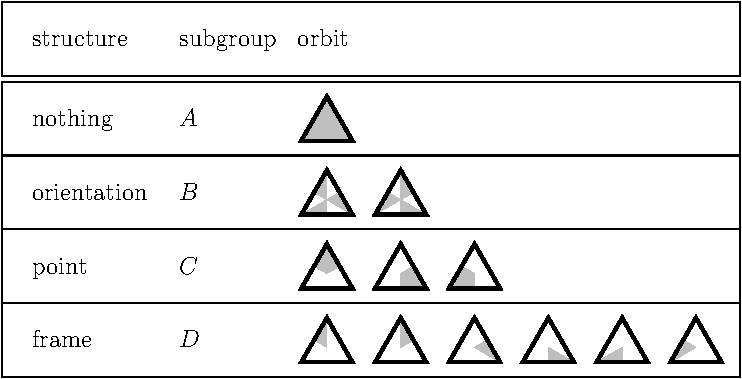
\includegraphics[]{pic-triangle-structures.pdf} 
\end{center}

The ordering of the table is misleading.
It's really a partially ordered set:
\begin{center}
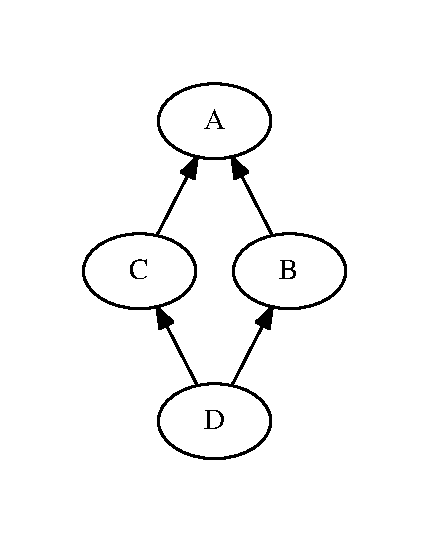
\includegraphics[width=0.3\columnwidth]{subgroups_s3.pdf} 
\end{center}

We next consider the conjunction (logical ``and'')
of two structures.
To keep track of the two structures when we combine them,
we use two colours, red and blue. 
\begin{center}
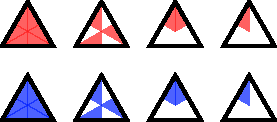
\includegraphics[]{pic-triangle-pairs.pdf} 
\end{center}
When we have two points that are not the same
this is what the orbit looks like:
\begin{center}
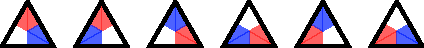
\includegraphics[]{pic-triangle-point-point-ne.pdf} 
\end{center}
This $G$-set is isomorphic to $D$. In other words,
two distinct (ordered) points are sufficient structure to pick
out a frame.
When we have two points that are the same
this is what the orbit looks like:
\begin{center}
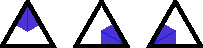
\includegraphics[]{pic-triangle-point-point-eq.pdf} 
\end{center}
The two points overlap which we show as purple. The resulting
$G$-set is isomorphic to the original $G$-set, $C.$
And this makes sense: ``two points that are identical''
is really no more structure than just having one point.

We therefore have the isomorphism:
$$
    C\times C \cong C + D.
$$

We can also examine the entire $G$-set $C\times C$ in a graphical way.
Here we show a matrix, with rows labelled by the orbit of one kind of
structure, and columns by the orbit of the other kind of structure.
The entries of the matrix then show the elements of the $G$-set $C\times C:$
\begin{center}
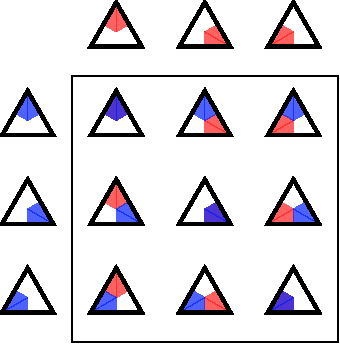
\includegraphics[]{pic-triangle-point-point-matrix.pdf} 
\end{center}
And we see the elements of this matrix break down into two
orbits. One orbit is on the diagonal,
and the other orbit is off the diagonal.
Once again we see that $C\times C \cong C+D.$
From this matrix we can also read off matrices for the two Hecke
operators corresponding to these two orbits:
$$
\left( \begin{array}{ccc}
1 & 0 & 0 \\
0 & 1 & 0 \\
0 & 0 & 1 \\
\end{array} \right),\ \ 
\left( \begin{array}{ccc}
0 & 1 & 1 \\
1 & 0 & 1 \\
1 & 1 & 0 \\
\end{array} \right).
$$

What we are doing here is (in great detail) examining how
two structures can \emph{geometrically relate} to each other.
For two points, there are two such relationships:
they can either be the same, or different.

\begin{samepage}
Here we show matrices for $B\times B\cong 2B$ and 
$B\times C\cong D:$
\begin{center}
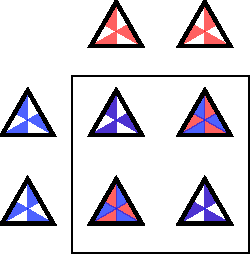
\includegraphics[]{pic-triangle-orient-orient-matrix.pdf} 
\ \ \ \ \ \ \ 
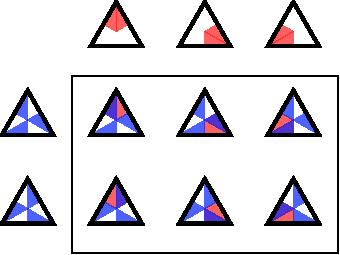
\includegraphics[]{pic-triangle-point-orient-matrix.pdf} 
\end{center}
\end{samepage}
In terms of geometric relationships: 
there are two ways for an orientation to relate to another
orientation (same or not), and there is only one way
for a point to relate to an orientation.

The most boring structure of all is the nothing structure $A$.
When we combine this structure with any other structure, we
just get the other structure.
For example, $A\times C\cong C:$
\begin{center}
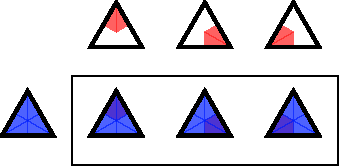
\includegraphics[]{pic-triangle-nothing-point-matrix.pdf} 
\end{center}

At the other end of the structures, 
when we combine a frame $D$ with any other structure,
we ``see everything''.
What this means is 
for some structure ($G$-set) $X$, we find that $D\times X$
breaks into $n$ copies of $D$, one for every element of $X$.
For example, $D\times C\cong 3D:$
\begin{center}
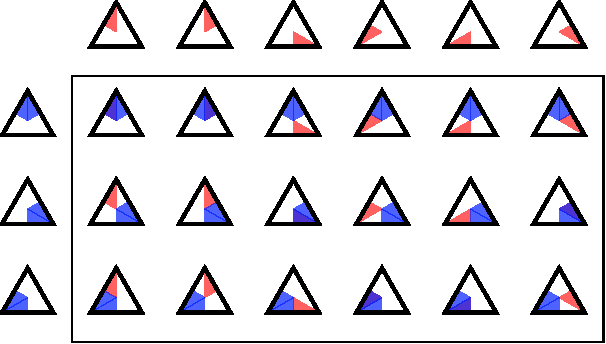
\includegraphics[]{pic-triangle-point-frame-matrix.pdf} 
\end{center}
It is a little hard to see, but there are three different
kinds of shapes in the above matrix, 
each of which is sufficient to serve as (isomorphic to) a frame.
And we see that there are three ways for a point to relate to
a frame. This makes sense: there are three points, and if we
have a frame then we can see each of these three points as distinct.

We summarize everything we know about 
multiplying these $G$-sets in the following table:
$$
\begin{array}{r|rrrr}
\times & A & B & C & D \\
\hline
A & A & B & C & D \\
B & B & 2B & D & 2D \\
C & C & D & C\thinplus D & 3D \\
D & D & 2D & 3D & 6D \\
\end{array}
$$

\subsection{Example: the square}

The dihedral group of order 8.

\begin{samepage}
\begin{center}
\begin{tabular}{ |l|l|c|c|c| }
\hline
structure & stabilizer subgroup & order & \#cosets & \#conjugates \\
\hline
\hline
nothing & $A=D_8$ &       8        &  1      &   1         \\
\hline
short axis& $B$ &       4        &  2      &   1         \\
\hline
long axis & $C$ &       4        &  2      &   1         \\
\hline
orientation & $D$ &       4        &  2      &   1         \\
\hline
point & $E$ &       2        &  4      &   2         \\
\hline
line  & $F$ &       2        &  4      &   2         \\
\hline
        & $G$ &       2        &  4      &   1         \\
\hline
frame & $H=\{1\} $ &       1        &  8      &   1         \\
\hline
\end{tabular}
\end{center}
\end{samepage}

\begin{center}
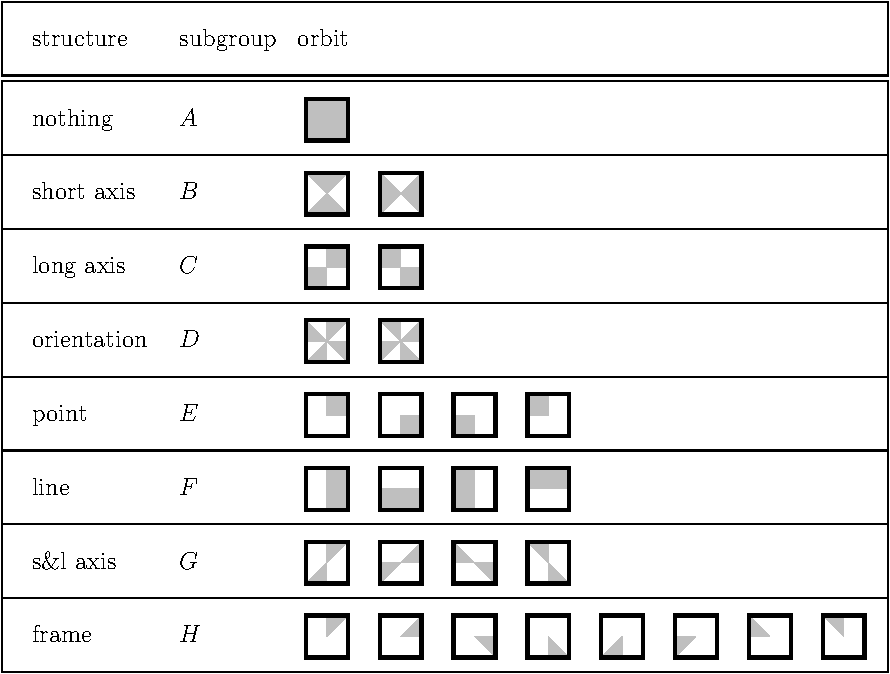
\includegraphics[]{pic-square-structures.pdf} 
\end{center}

\begin{center}
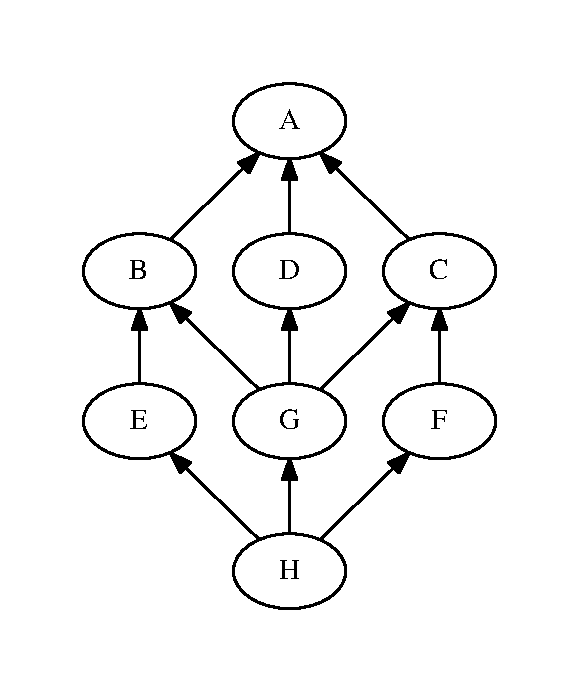
\includegraphics[width=0.4\columnwidth]{subgroups_d8.pdf} 
\end{center}

%G: 8
%equ: [8]
%equ: [4]
%equ: [4]
%equ: [4]
%equ: [2, 2]
%equ: [2, 2]
%equ: [2]
%equ: [1]
%total: 8
%A subgroup order = 8, number of cosets = 1
%B subgroup order = 4, number of cosets = 2
%C subgroup order = 4, number of cosets = 2
%D subgroup order = 4, number of cosets = 2
%E subgroup order = 2, number of cosets = 4
%F subgroup order = 2, number of cosets = 4
%G subgroup order = 2, number of cosets = 4
%H subgroup order = 1, number of cosets = 8


$$
\begin{array}{r|rrrrrrrr}
\times & A & B & C & D & E & F & G & H \\
\hline
A & A & B & C & D & E & F & G & H \\
B & B & 2B & G & G & 2E & H & 2G & 2H \\
C & C & G & 2C & G & H & 2F & 2G & 2H \\
D & D & G & G & 2D & H & H & 2G & 2H \\
E & E & 2E & H & H & 2E\thinplus H & 2H & 2H & 4H \\
F & F & H & 2F & H & 2H & 2F\thinplus H & 2H & 4H \\
G & G & 2G & 2G & 2G & 2H & 2H & 4G & 4H \\
H & H & 2H & 2H & 2H & 4H & 4H & 4H & 8H \\
\end{array}
$$


\subsection{Example: $S_4$}

%G: 24
%equ: [24]
%equ: [12]
%equ: [8, 8, 8]
%equ: [6, 6, 6, 6]
%equ: [4, 4, 4]
%equ: [4]
%equ: [4, 4, 4]
%equ: [3, 3, 3, 3]
%equ: [2, 2, 2, 2, 2, 2]
%equ: [2, 2, 2]
%equ: [1]
%total: 11
%A subgroup order = 24, number of cosets = 1
%B subgroup order = 12, number of cosets = 2
%C subgroup order = 8, number of cosets = 3
%D subgroup order = 6, number of cosets = 4
%E subgroup order = 4, number of cosets = 6
%F subgroup order = 4, number of cosets = 6
%G subgroup order = 4, number of cosets = 6
%H subgroup order = 3, number of cosets = 8
%I subgroup order = 2, number of cosets = 12
%J subgroup order = 2, number of cosets = 12
%K subgroup order = 1, number of cosets = 24


$$
\begin{array}{r|rrrrrrrrrrr}
\times & A & B & C & D & E & F & G & H & I & J & K \\
\hline
A & A & B & C & D & E & F & G & H & I & J & K \\
B & B & 2B & F & H & J & 2F & J & 2H & K & 2J & 2K \\
C & C & F & C\thinplus F & I & E\thinplus J & 3F & G\thinplus J & K & I\thinplus K & 3J & 3K \\
D & D & H & I & D\thinplus I & 2I & K & K & H\thinplus K & 2I\thinplus K & 2K & 4K \\
E & E & J & E\thinplus J & 2I & 2E\thinplus K & 3J & J\thinplus K & 2K & 2I\thinplus 2K & 2J\thinplus 2K & 6K \\
F & F & 2F & 3F & K & 3J & 6F & 3J & 2K & 3K & 6J & 6K \\
G & G & J & G\thinplus J & K & J\thinplus K & 3J & 2G\thinplus K & 2K & 3K & 2J\thinplus 2K & 6K \\
H & H & 2H & K & H\thinplus K & 2K & 2K & 2K & 2H\thinplus 2K & 4K & 4K & 8K \\
I & I & K & I\thinplus K & 2I\thinplus K & 2I\thinplus 2K & 3K & 3K & 4K & 2I\thinplus 5K & 6K & 12K \\
J & J & 2J & 3J & 2K & 2J\thinplus 2K & 6J & 2J\thinplus 2K & 4K & 6K & 4J\thinplus 4K & 12K \\
K & K & 2K & 3K & 4K & 6K & 6K & 6K & 8K & 12K & 12K & 24K \\
\end{array}
$$

\subsection{Example: $\GL(3, 2)$}




\section{Bibliographic notes}

Group actions with applications to group theory: \cite{ConradGroup,ConradTransitive}.

See \cite{Dress1971}.


\bibliography{refs}{}
\bibliographystyle{abbrv}



\end{document}



